\section{Critical Path Scheduler (CPATH)}
\label{sec.scheduling.cpath}
\begin{figure}[tr]
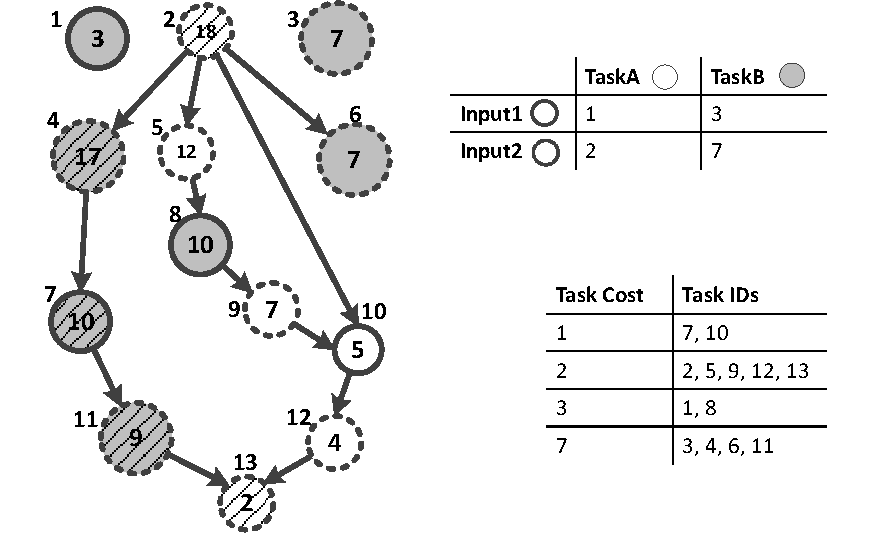
\includegraphics[width=\columnwidth]{images/cpath_priorities.pdf} 
\centering
\caption{Priority assignment with CPATH taking into account the task costs. Task costs are assumed known and are shown in the tables.}
\label{cpath}
\vspace{-0.5cm}
\end{figure}


The Critical Path scheduler (CPATH) dynamically detects the critical path of the TDG.
Like CATS, CPATH separates tasks into two groups: critical and non-critical tasks.
The detected critical tasks are executed by the fast cores in the system and non-critical tasks are executed by slow cores.
The difference with CATS is the algorithm for critical path detection.
CPATH takes into account the task execution time, about which CATS is unaware.
To do so, CPATH implements a more complex and accurate critical path detection algorithm that takes into account task execution time.

CPATH scheduler consists of three steps:
%\begin{itemize}

\textbf{Task prioritization}: this step takes place when a task is finishing its execution. This is different than CATS since at the end of a task execution the algorithm may record the task execution time (task cost).
%might track a new (unknown) task cost. 
According to the discovered task cost CPATH assigns priorities to tasks by traversing the TDG from top to bottom, introducing the cost of \textit{O($2n^2$)}, where \textit{$n$} is the number of tasks.

\textbf{Task submission}: when a task becomes \textit{ready}, it is submitted to a \textit{ready queue}. At this point, CPATH decides whether or not the task is \textit{critical} and inserts it in the corresponding ready queue. This step has only slight implementation differences with CATS and complexity of \textit{O($n$)}.

\textbf{Task-to-core assignment}: this step is identical to CATS.
% and supports the same work stealing mechanisms.

%\end{itemize}

\subsection{Task Prioritization}
%explanation of the slist (successors' list)

Each task of the TDG keeps a list with its successors (\textit{slist}).
This list is being built when an edge (dependency between two tasks) is added in the TDG.
So when a task dependency occurs, the corresponding successor task is added in the \textit{slist} of its predecessor.
For example, on Figure~\ref{cpath}, when the dependency between tasks 2 and 4 occurs, the \textit{slist} of task number 2 becomes \{4\}. 
This goes on for all the added edges of the TDG, therefore when the edge~2$\rightarrow$5 is inserted in the TDG, the task number 5 is inserted in the \textit{slist} of task number 2; so the \textit{slist} of task number 2 becomes \{4, 5\}.

The goal of this step is to assign priorities based on the \textit{bottom cost} of the tasks of the TDG.
We define the \textit{bottom cost} of a node on a directed acyclic graph as the maximum estimated time in the dependency chains from this node to a leaf node.
So the main difference between the \textit{bottom level} and the \textit{bottom cost} is the consideration of the estimated time.

Figure~\ref{cpath} is used to describe the priority assignment with CPATH.
The specific TDG contains tasks of two different types and two different input sizes.
Node color shows the different task types and the outline of the circle (dashed or solid) shows the different input sizes.
The upper table in Figure~\ref{cpath} indicates the execution time of the tasks according to their type and input size.
The algorithm assumes that task instances of the same type with the same input size have the same (or very similar) execution time.
To track this information, CPATH discovers the cost of every possible task type-input size duple (tt-is duple) that appears on the TDG.
The numbers inside the nodes show the bottom cost-based priorities that CPATH assigns and the numbers outside the nodes show their task ID.


%This task type-input size duple is denoted as tt-is and the algorithm assumes that the task with the same tt-is have the same execution time.
%So the execution time of the tasks differs according to the task type-input size duple (\texttt{tt-is} duple).
%CPATH discovers the cost for all the tt-is pairs and prioritizes the tasks according to their \textit{bottom cost} as shown on Figure~\ref{cpath}.
%The bottom cost of a node is equal to the maximum estimated time in the dependency chains from this node to a leaf node.

The task prioritization step takes place every time a task finishes execution. 
CPATH uses a vector to store task costs and keeps one entry per tt-is.
Because CPATH needs to discover the unbiased critical path of the TDG, it uses one of the core types as reference to track the task costs.
%So at the beginning of the execution tasks are executed on one of the core types during this cost-learning phase.
In our experiments we chose to use as reference the fast cores since this way the learning phase (that is, the phase where CPATH discovers the task costs) becomes shorter.
To avoid wrong task cost prediction of future tasks, CPATH ignores the first execution of each tt-is because usually it takes more time. 
\begin{lstlisting}[float, emph={for,in,void,if,return,updatePriorities,non_critical_queue, critical_queue,submit_task}, captionpos=b, caption={Pseudo-code for taskExit, the function called by the cores used as reference for tracking the task costs},label=cpathExit, emph={[2]mat}, emphstyle={[2]}, aboveskip={0\baselineskip}, frame=tb, belowskip={-0.4cm}]
1 void taskExit (task* finished) {
2  if( stateOf(finished) == init ) {
3    finished->state = in_progress;
4    return;
5  }
6  if( stateOf(finished) == in_progress ) {
7    timesSet[finished] = finished->execTime;
8    finished->state = tracked;
9  }
10 task* succ;
11 for( succ in finished->successors ) 
12   if( numPredecessorsOf(succ) == 1 ) {
13     lock();
14     if( succ $\notin$ entryNodes ) 
15       entryNodes->push(succ);
16       unlock();
17   }
18 list<task>* updatedList = new list<task>();
19 for( node in entryNodes) 
20   updatePriorities(node, updatedList);
21 for( node in updatedList ) 
22    node->unsetUpdated();
23}
\end{lstlisting}

Listings \ref{cpathExit} and \ref{cpathUpdate} show how the critical path scheduler performs task prioritization.
Whenever a task finishes execution on one of the cores used as reference (here: fast cores) the runtime makes a call to the \texttt{taskExit} routine shown in Listing~\ref{cpathExit}.
At this point, the runtime is aware of the execution time of the finished task.
This function has the responsibility to update the known task costs and also perform the prioritization of the tasks on the TDG.
The prioritization is done by the \texttt{updatePriorities} function of Listing~\ref{cpathUpdate}. 
This function is responsible for TDG traversal.

The \texttt{taskExit} function in Listing~\ref{cpathExit} takes as an argument the task that has just finished. 
In order to keep track of whether the execution time of the tt-is has been discovered we implement a small finite state machine within this stage.
Every tt-is has three possible states. 
The initial state is the \texttt{init} state; this means that the specific tt-is has not yet been executed so its execution time is totally unknown.
When a tt-is is executed for the first time its state changes from \texttt{init} to 
\texttt{in$\_$progress}. 
This means that a task of this tt-is has been executed once, but CPATH ignores this cost because the first instance may not be representative due to cold start effects and one sample may not be enough history for prediction.
While the tt-is of a node is in \texttt{init} or \texttt{in$\_$progress} state its execution time is considered to be 1.
%we have to ignore this execution because usually it takes too long and is not representative.
After the second execution of a tt-is the state of it becomes \texttt{tracked} meaning that the execution time has been tracked and can be used for the computation of the priorities.
%If the node does not have a known execution cost tracked, we consider its execution time to be 1.

After the first checks of the tt-is state (lines 2-9 of Listing~\ref{cpathExit}) the algorithm traverses the \textit{slist} of the finished task and searches for the successors that become ready by the end of the execution of this task.
This is identified by the fact that the ready-to-be successors have one unique (remaining) predecessor (e.g. the just finished task).
These successors are inserted in the \texttt{entryNodes} list (lines 11-16 of Listing~\ref{cpathExit}).
For each one of the entry nodes the \texttt{updatePriorities} function is called (line 19 of Listing~\ref{cpathExit}); this performs a top to bottom traversal of the TDG and updates the priorities.

\begin{lstlisting}[float, emph={for,in,void,if,return,non_critical_queue, critical_queue,submit_task}, captionpos=b, caption={Pseudo-code for task prioritization with CPATH},label=cpathUpdate, emph={[2]mat}, emphstyle={[2]}, aboveskip={0\baselineskip}, frame=tb, belowskip={-0.5cm}]
1 int updatePriorities (task* currT, list* updated) {
2   if( currT == NULL )  return 0;
3   if( isVisited(currT) )  
4     return priorityOf(currT);
5   successors = currT->successors;
6   int maxSucc = -1;
7   bool succVisited = true;
8  
9   for(succ in successors) {
10    int succPriority;
11    //Avoid double update
12    if( !isUpdated(succ) || !isVisited(succ) ) {
13      succPriority = updatePriorities(succ, updated);
14      succ->setUpdated();
15      updated->push(succ);
16    }
17    else 
18      succPriority = priorityOf(succ);
19    if(succPriority > maxSucc)
20       maxSucc = succPriority;
21    succVisited = succVisited && isVisited(succ);   
22  }
23  if( timeIsTracked(currT) ) {
24    currT->priority = (maxSucc + timesSet[currT]);
25    if(succVisited && groupOf(currT) < twDetected) 
26      currT->setVisited();
27  }  
28  else
29    currT->priority = maxSucc + 1;
30    
31  return priorityOf(currT);  
32}
\end{lstlisting}

Due to the properties of the top-to-bottom TDG traversal, the algorithm has to make sure that every node is prioritized only once per \texttt{updatePriorities} call.
This is controlled by checking the \texttt{updated} flag of each node of the TDG.
To visualize this situation let us assume that task number 2 of the TDG on Figure~\ref{cpath} finishes.
Then the \texttt{entryNodes} list contains three tasks that will start the update: \{4, 5, 6\}.
The update that starts from task number 4 marks tasks 4, 7, 11 and 13 as updated.
Then, during the update of task number 5, the algorithm knows that task 13 has already been prioritized during the same update so there is no need to apply the algorithm at this node again.
This example does not show too much optimization because in this case the update of only one node is saved, but in real applications this node could have numerous successors for whom the priority update would be a large overhead.

The raising of the \texttt{updated} flag is something temporal and is only used for helping the prioritization of a single update.
There are cases when CPATH needs to raise a permanent flag in order to mark that the priority of the task will not change again in the future, e.g. it is the final priority.
This happens when the execution times of all the tt-is that appear on the TDG have been discovered, for the tasks that their priorities are up to date.
To mark these tasks CPATH uses the \texttt{visited} flag.
If a task is \texttt{visited}, there is no need to get prioritized again.
To clarify this, let us assume that in Figure~\ref{cpath} the task costs of the tt-is TaskA-Input2 and TaskB-Input2 are known.
During the next prioritization, tasks 11 (TaskB-Input2), 12 (TaskA-Input2) and 13 (TaskA-Input2) in the TDG will be set as visited, because their priorities consist of the sum of known task execution times and they do not have any successors (with unknown execution times).
So, an additional priority update in cases like this is redundant.
%So, the algorithm does not need to visit these nodes again on the current update, nor on a future priority update.


%Moreover, CPATH prioritization needs to make sure that the priority of a to-be-updated node is not the final priority.
%In case that the priority of a node is final then there is no need for updating this node.
%To perform this check, CPATH checks the \texttt{visited} flag of every node, which tells if the priority of the node is final.
%To understand what a final priority is, let's assume that CPATH has discovered the task costs of the tt-is TaskA-Input2 and TaskB-Input2 on the Figure~\ref{cpath}.
%This means that the tasks 11, 12 and 13 of the TDG are visited, because their priorities are not going to change since they consist of the sum of known task execution times and they don't have any successors.
%So, the algorithm does not need to visit these nodes again not on the current update, neither on a future priority update.



%For example, in Figure~\ref{cpath}


%Because one node might get updated more than once through different possible paths, we optimize the procedure by keeping the \texttt{updated} flag. 
%This flag tells whether the node has been updated during the prioritization that caused the exit of the same task. 
%This way duplicate updates on a single task exit are skipped and we make sure that the nodes are updated only once.
%At the end of this routine the updated flag is being unset because the nodes have to be updated in case a new task cost is discovered in a future task exit.

Listing~\ref{cpathUpdate} shows what happens during the the update of one entry node.
The arguments of this function are \texttt{currT}, that is the entry node being updated, and \texttt{updated}, that is the list with the updated nodes. 
This list is being filled throughout the priority update in order to unset the updated flag later.
The lines 2-4 of Listing~\ref{cpathUpdate} perform the checks that would cause the traversal to finish.
If the node is not visited, then the algorithm traverses its successors.
Note that, at this point, there is no check for updated flag, since tasks in the \texttt{entryNodes} are unlikely to be updated. 
Updated nodes can only be discovered through recursive calls and this check is performed later.
%this cannot happen from the entryNodes, only from recursive calls which is checked later.
If a successor is updated or visited, the priority update is skipped for the reasons explained above. 
Otherwise, the \texttt{updatePriorities} is called recursively for the current successor.
This happens until we detect a node that is updated, visited or is a leaf node (node with no successors) of the TDG.
When the algorithm reaches a node ready for update it calculates its priority by summing the highest priority of its successors to the execution time, if known, of the current node (lines 24, 29).
Finally, the visited flag of the task is being updated. 

There are three conditions that mark a task as visited: \textit{(a)} if its execution time is known (line 23),  \textit{(b)} if \textbf{all} of its successors are visited (line 25) or \textit{(c)} if we have encountered a taskwait (barrier) after the creation of this task (line 25).
%To mark a node as visited we have to check the following:
%\begin{itemize}
%\item If the execution time tracked of this tt-is is known (line 23)
%\item If \textbf{all} of the task's successors are visited (line 25)
%\item If we have encountered a taskwait (barrier) after the creation of this task (line 25)
%\end{itemize}
%In addition to the updated flag, the algorithm uses the \texttt{visited} flag.
%The algorithm is not using only the updated flag to mark the updates; each node in the TDG can be marked as \texttt{visited} as well.
%The \texttt{visited} flag tells to the algorithm that the node has a valid and unchangeable priority.
%This shows that the priorities of all the descendants of this task have valid execution times tracked and their priorities are computed according to these final values. 
%Thus there is no need to traverse the successors of a visited node and this is an important optimization of the algorithm.
%
%As described, the lines 2-4 of Listing~\ref{cpathUpdate} perform the checks that would cause the traversal to finish.
%If the node is not visited, then the algorithm traverses its successors.
%If a successor is updated or visited the update of priorities is skipped. 
%Otherwise, the \texttt{updatePriorities} is called recursively using the current successor as an entry node.
%This happens until we find a node that has been updated or is visited or a leaf node (node with no successors) of the TDG.
%When the algorithm reaches a node ready for update it calculates its priority by summing the highest priority of its successors with the execution time, if known, of the current node (lines 24, 29).
%If the node does not have a known execution cost tracked, we consider its execution time to be 1.
%Finally, the visited flag of the updated task is being updated. 
%To mark a node as visited we have to check the following:
%\begin{itemize}
%\item If the execution time tracked of this tt-is is valid
%\item If \textbf{all} of the task's successors are visited
%\item If we have encountered a taskwait after the creation of this task
%\end{itemize}
The last condition confirms that it is safe to mark this task as visited as there will be no future successors of this task on the current TDG. 
%The reason behind the last condition is that if we have encountered a taskwait \textbf{after} the creation of this task this means that there will be no future successors on the current TDG. 
%Thus, we do not need to worry about setting priorities on tasks that reside below the visited tasks of the TDG.
To track this information we use an atomic variable, \texttt{twDetected}, which is increased every time a taskwait is encountered.
At creation time, each task is assigned a group ID which is the value of the \texttt{twDetected} at that moment.
%This way the tasks are separated into groups according to the detected taskwaits.
%At creation time, tasks are separated into groups according to the detected taskwaits by assigning as group ID the value of the \texttt{twDetected} at that moment.
If the group ID of a task is less than the current \texttt{twDetected} value then this means that a taskwait has occurred after the creation of this task.

\subsection{Task Submission} 
The task submission is implemented using the same \texttt{critical} and \texttt{non-critical} ready queues as in CATS.
Listing~\ref{submission} can be used to describe the task submission of CPATH.
The only modification needed is in the condition of the lines 6 and 7 of Listing~\ref{submission}.
In addition to the \texttt{maxPriority}, CPATH keeps track of the \texttt{maxExecTime} which is the cost of the last discovered critical task.
CPATH extends the condition of the critical task consideration by checking whether the priority of the current task is equal to \texttt{maxPriority} - \texttt{1} or if it is equal to \texttt{maxPriority} - \texttt{maxExecTime}.
Moreover, the value of \texttt{maxExecTime} is updated accordingly to the \texttt{maxPriority}.

\subsection{Task-to-Core Assignment}
Task-to-core assignment in CPATH is identical to CATS as described in Section~\ref{sec.cats.assignment}. 
It takes place dynamically and in parallel to the previous steps.
Depending on the core type, whenever a core becomes idle it retrieves a task from its corresponding ready queue; fast cores are responsible for the execution of the tasks in the critical queue and slow cores for the tasks in the non-critical queue.
Each ready queue is shared among the cores of the same type so there is no need for work stealing among cores of the same type. 
Finally, as with CATS, the work-stealing mechanism prevents load imbalance by allowing big cores to steal work from the little cores.




